\documentclass[11pt,a4paper]{article}

% --- Packages ---
\usepackage[top=2.5cm,bottom=2.5cm,left=2.5cm,right=2.5cm]{geometry}
\usepackage{amsmath,amssymb,amsfonts,amsthm}
\usepackage{booktabs,multirow,tabularx,array}
\usepackage{graphicx}
\usepackage{float}
\usepackage{caption,subcaption}
\usepackage{hyperref}
\usepackage{microtype}
\usepackage{cite}
\usepackage{xurl}
\usepackage{url}
\usepackage{xcolor}
\usepackage{iftex}

% --- Font Configuration (XeLaTeX with Ethiopic Script Fallback) ---
\ifXeTeX
  \usepackage{fontspec}
  \usepackage{ucharclasses}
  \setmainfont{Times New Roman}
  \newfontfamily\ethiopicfont{Nyala}
  \setTransitionsFor{Ethiopic}{\ethiopicfont}{\normalfont}
\else
  \usepackage[utf8]{inputenc}
  \usepackage[T1]{fontenc}
\fi

\hypersetup{
    colorlinks=true,
    linkcolor=blue!70!black,
    citecolor=blue!70!black,
    urlcolor=blue!70!black
}

% --- Custom formatting ---
\setlength{\parskip}{0.5em}
\setlength{\parindent}{0pt}

\title{\textbf{\Large Evaluating Conversational Intelligence in Large Language Models\\Using English--Amharic Code-Switching}}

\author{
    \textbf{Kindie Alebachew Tsega}$^{1,2*}$, 
    \textbf{Durga Prasad Sharma}$^{1}$, 
    \textbf{Mesay Samuel Gondere}$^{1}$, \and
    \textbf{Mohammed Abebe Yimer}$^{1}$
}

\date{
    \small
    $^{1}$Faculty of Computing and Software Engineering, Arba Minch Institute of Technology, Arba Minch University, P.O. Box 21, Arba Minch, Ethiopia\\
    $^{2}$Department of Computer Science, Debre Tabor University, P.O. Box 272, Debre Tabor, Ethiopia\\[1ex]
    $^{*}$Corresponding author: \texttt{besukind@gmail.com}
}

\begin{document}

\maketitle

\begin{abstract}
Large language models (LLMs) have achieved remarkable conversational capabilities in high-resource monolingual domains. However, their ability to sustain intelligent multi-turn interactions in low-resource bilingual and code-switched contexts remains critically understudied. This paper presents an extensive empirical investigation into conversational intelligence across English--Amharic code-switching, a socio-linguistically rich Afroasiatic language pair characterized by stark morphological complexity, distinct writing scripts (Latin vs.\ Ge'ez), and asymmetric pre-training data representation. To rigorously evaluate current AI systems, we construct and validate \textbf{EthioSwitch-Bench}, an expanded benchmark comprising 2,000 multi-turn dialogues (10,000 conversational turns) spanning 15 diverse communicative domains, paired with a gold-standard hand-crafted test set of 30 dialogues. Using this corpus, we benchmark five architecturally diverse language models: GPT-4, mBERT-fine-tuned, mT5-Large, LLaMA-2-7B, and BLOOM-7B. We formulate four central research questions regarding contextual coherence (RQ1), semantic consistency under code-switch frequency variation (RQ2), switch-point detection accuracy across language transition directions (RQ3), and conversational fluency parity across language dominance contexts (RQ4). Our empirical findings demonstrate that GPT-4 achieves the highest contextual coherence ($4.78 \pm 0.34$) and overall lexical fidelity (BLEU 0.6086, ROUGE-L 0.8634), significantly outperforming open-weight monolingual and cross-lingual baselines (Welch's $t = 142.94$, $p < 0.001$, Cohen's $d = 4.52$). Supervised task-specific fine-tuning on mBERT yields remarkable switch-point detection capability (Switch F1 = 0.7730), matching GPT-4 (0.7745) and surpassing zero-shot baselines which fail entirely (Switch F1 = 0.0000). Furthermore, we uncover a pronounced directional asymmetry: all multilingual models achieve substantially higher switch accuracy when transitioning from English into Amharic ($0.8327 \pm 0.3733$) than during return transitions into English ($0.6388 \pm 0.4804$, $p < 0.001$), reflecting subword script fragmentation and matrix language syntactic constraints. Finally, correlation analyses reveal that increasing code-switching frequency monotonically degrades semantic consistency (Spearman's $\rho = -0.8319$, $p < 0.001$), whereas conversational fluency remains statistically equivalent across English-dominant and Amharic-dominant contexts (paired $t = 0.4437$, $p = 0.657$). We release the annotated EthioSwitch-Bench corpus, evaluation pipeline, and reproducibility suite to accelerate future research in linguistically equitable conversational AI.
\end{abstract}

\textbf{Keywords:} English--Amharic code-switching; conversational intelligence; large language models; low-resource NLP; multilingual benchmarks; EthioSwitch-Bench; matrix language frame; switch-point detection.

\vspace{1em}
\hrule
\vspace{1.5em}

% =========================================================================
% 1. INTRODUCTION
% =========================================================================
\section{Introduction}

The emergence of transformer-based large language models (LLMs) has fundamentally transformed conversational artificial intelligence, enabling machines to produce fluent, context-sensitive responses across complex multi-turn dialogues \cite{achiam2023gpt4, touvron2023llama2, vaswani2017attention}. Despite extraordinary breakthroughs in high-resource standard languages, state-of-the-art conversational agents exhibit severe performance degradation when confronted with non-standard linguistic phenomena, most notably \textit{code-switching} (CS)---the fluid alternation between two or more languages or linguistic varieties within a single communicative exchange \cite{grosjean2010bilingual, poplack1980sometimes, sitaram2019survey}. Code-switching is not an anomalous linguistic defect; rather, it represents the default communicative mode for hundreds of millions of multilingual speakers across the Global South, serving vital pragmatic, social, and cultural functions \cite{myersscotton1993duelling, muysken2000bilingual}.

Evaluating conversational intelligence in code-switched dialogues presents profound scientific and computational hurdles that surpass standard monolingual benchmarks. A truly intelligent conversational agent must not merely translate words verbatim; it must master four tightly coupled capabilities:
\begin{enumerate}
    \item \textbf{Contextual and Semantic Coherence:} Tracking conversational state across multi-turn exchanges while maintaining topical integrity and contextual grounding across abrupt language transitions.
    \item \textbf{Syntactic and Structural Integrity:} Adhering to the intricate morphosyntactic constraints governing grammatical switch boundaries, preventing ungrammatical clause structures as formalised by the Matrix Language Frame (MLF) model \cite{myersscotton1993duelling}.
    \item \textbf{Linguistic and Script Alternation Dynamics:} Operating across asymmetric orthographic scripts without succumbing to subword tokenizer fragmentation or byte-fallback collapse \cite{ahia2021tokenization}.
    \item \textbf{Pragmatic and Sociolinguistic Naturalness:} Producing conversational turns that mirror the socio-pragmatic expectations, colloquial idioms, and affective undertones of real bilingual communities \cite{grosjean2010bilingual}.
\end{enumerate}

Nowhere are these computational challenges more pronounced than in conversational exchanges pairing English with Amharic. Amharic, an Afroasiatic language of the Semitic branch spoken by over 32 million people primarily in Ethiopia, differs fundamentally from English across every linguistic dimension \cite{leyew1998amharic, yimam2021amharic}. Structurally, Amharic exhibits an agglutinative root-and-pattern (templatic) morphology, a Subject--Object--Verb (SOV) default word order, and a rich system of verbal clitics and prepositional affixes, in stark contrast to English's isolating morphosyntax and canonical Subject--Verb--Object (SVO) typography \cite{alebachew2024african, andersland2024amharic}. Orthographically, Amharic is written in the Ethiopic (Ge'ez) abugida script, where each character denotes a consonant-vowel syllable, whereas English uses the Latin alphabet. In urban Ethiopian centers and diaspora communities, bilingual professionals, university students, and technology users continuously engage in conversational code-switching, effortlessly weaving English technical terminology, greetings, and colloquial phrases into Ge'ez-scripted Amharic discourse.

Despite its vibrant socio-cultural reality, English--Amharic code-switching represents an extreme low-resource NLP scenario \cite{adebara2022african, tonja2023ethiopian}. Existing conversational benchmarks (e.g., MultiWOZ \cite{budzianowski2018multiwoz}, DailyDialog \cite{li2017dailydialog}) are predominantly English-only. Cross-lingual benchmarks such as XGLUE \cite{liang2020xglue} and XTREME \cite{hu2020xtreme} evaluate downstream classification or translation but omit code-switched multi-turn dialogue. Code-switching corpora (such as LinCE \cite{aguilar2020lince} and GLUECoS \cite{khanuja2020gluecos}) focus almost exclusively on high-resource language pairs (Spanish--English, Hindi--English) or single-turn syntactic classification tasks, leaving Afroasiatic, multi-script conversational dynamics completely unaddressed.

To bridge this fundamental research gap, this paper introduces a comprehensive empirical benchmarking framework and presents an exhaustive evaluation of state-of-the-art LLMs on English--Amharic code-switched conversational intelligence. We systematically formulate and investigate four key research questions:
\begin{itemize}
    \item \textbf{RQ1 (Contextual Coherence \& Fidelity):} How effectively do modern closed-source and open-weight LLMs maintain contextual coherence, semantic relevance, and lexical fidelity during multi-turn English--Amharic code-switched conversations?
    \item \textbf{RQ2 (Switch Frequency \& Consistency Degradation):} Does increasing code-switching frequency within a dialogue turn induce a systematic degradation in model semantic consistency and discourse stability?
    \item \textbf{RQ3 (Transition Directionality Asymmetry):} Does model switch-point prediction accuracy differ significantly based on the direction of language transition (English $\rightarrow$ Amharic vs.\ Amharic $\rightarrow$ English), and what structural factors govern this asymmetry?
    \item \textbf{RQ4 (Language Dominance \& Fluency Parity):} Does conversational fluency exhibit parity across English-dominant versus Amharic-dominant turns, or do models display an asymmetric bias toward the high-resource Latin-scripted language?
\end{itemize}

This study delivers five distinct scientific and technical contributions:
\begin{enumerate}
    \item \textbf{EthioSwitch-Bench Corpus:} We construct and validate \textit{EthioSwitch-Bench}, an expanded conversational benchmark of 2,000 multi-turn dialogues (10,000 conversational turns) balanced across 15 communicative domains, three code-switching frequency tiers, and three language dominance contexts, accompanied by a rigorously annotated gold test set of 30 dialogues (150 turns).
    \item \textbf{Multi-Architectural Empirical Benchmark:} We conduct the first systematic multi-paradigm evaluation comparing proprietary frontier models (GPT-4), task-specific fine-tuned encoders (mBERT), multilingual sequence-to-sequence transformers (mT5-Large), and open-weight autoregressive LLMs (LLaMA-2-7B, BLOOM-7B).
    \item \textbf{Formalized Multi-Dimensional Evaluation Framework:} We implement a unified evaluation pipeline integrating surface lexical metrics (BLEU-4, ROUGE-L), deep contextual embeddings (BERTScore F1, LaBSE cosine similarity), fine-grained syntactic metrics (Switch Precision, Recall, and F1), language modeling uncertainty (Perplexity), and rigorous human qualitative ratings.
    \item \textbf{Empirical Discovery of Directional and Tokenizer Asymmetry:} We mathematically uncover and validate a statistically significant directional asymmetry ($p < 0.001$), proving that models predict English-to-Amharic switches far more accurately than return switches, and we mechanistically trace open-model failure to subword tokenizer fertility disparities.
    \item \textbf{Open-Source Scientific Reproducibility Suite:} We release the complete dataset, automated validation scripts, evaluation pipelines, and figure generation routines under permissive open-source licenses to foster equitable research in African and low-resource multilingual conversational AI.
\end{enumerate}

% =========================================================================
% 2. RELATED WORK & THEORETICAL FOUNDATIONS
% =========================================================================
\section{Related Work and Theoretical Foundations}

\subsection{Multilingual and Cross-Lingual Language Models}
The progression from monolingual transformers \cite{vaswani2017attention} to massively multilingual models has catalyzed cross-lingual NLP. Early masked language models like mBERT \cite{devlin2019bert} and XLM-RoBERTa \cite{conneau2020xlmr} demonstrated that shared subword vocabularies across 100+ languages foster cross-lingual alignment in hidden representation spaces. Concurrently, encoder-decoder architectures such as mT5 \cite{xue2021mt5} extended multilingual pre-training across the mC4 corpus. More recently, open autoregressive LLMs such as BLOOM-7B \cite{lescao2022bloom} and LLaMA-2-7B \cite{touvron2023llama2}, alongside closed frontier systems like GPT-4 \cite{achiam2023gpt4}, have exhibited strong zero-shot and few-shot in-context learning. However, as documented by Adebara et al.\ \cite{adebara2022african} and Ahuja et al.\ \cite{ahuja2023mega}, African languages remain severely marginalized during pre-training, representing less than 0.1\% of Web crawled corpora. Consequently, their contextual representations in open-weight models suffer severe spatial distortion.

\subsection{Sociolinguistic Foundations of Code-Switching}
Sociolinguists categorize code-switching into three primary structural patterns \cite{muysken2000bilingual, poplack1980sometimes}: (i) \textit{tag-switching} (inserting an emblematic tag or greeting into another language), (ii) \textit{inter-sentential switching} (alternating languages at sentence or clause boundaries), and (iii) \textit{intra-sentential switching} (switching within a single clause or syntactic phrase). Intra-sentential switching imposes the highest cognitive and computational burden, as it requires simultaneous adherence to the grammatical systems of both participating languages.

The theoretical bedrock of modern computational code-switching is Myers-Scotton's \textbf{Matrix Language Frame (MLF) model} \cite{myersscotton1993duelling, myersscotton2002contact}. The MLF posits that in any code-switched clause, one language functions as the \textit{Matrix Language} (ML), providing the morphosyntactic frame (phrase structure rules, word order, and system morphemes), while the other language operates as the \textit{Embedded Language} (EL), contributing content morphemes. The MLF establishes two inviolable principles:
\begin{enumerate}
    \item \textbf{The Morpheme Order Principle:} In ML+EL constituents, morpheme order must conform strictly to the surface ordering rules of the Matrix Language.
    \item \textbf{The System Morpheme Principle:} All structurally active system morphemes (inflectional affixes, agreement clitics, determiners, copulas) must originate from the Matrix Language.
\end{enumerate}
In English--Amharic code-switching, Amharic almost invariably acts as the Matrix Language in informal and professional discourse, supplying verbal prefixes, subject/object agreement clitics, and SOV ordering, while English supplies EL noun phrases, technical terms, and verbal roots \cite{leyew1998amharic, alebachew2024african}.

\subsection{Conversational Benchmarks and the Low-Resource Evaluation Gap}
Multi-turn conversational evaluation has matured through standard benchmarks such as Persona-Chat \cite{zhang2018personachat}, MultiWOZ \cite{budzianowski2018multiwoz}, DailyDialog \cite{li2017dailydialog}, EmpatheticDialogues \cite{rashkin2019empathetic}, and BlendedSkillTalk \cite{smith2020blended}. However, these datasets are strictly monolingual English. While multilingual benchmarks such as GLUE \cite{wang2018glue}, XGLUE \cite{liang2020xglue}, and XTREME \cite{hu2020xtreme} evaluate cross-lingual classification and QA, they do not include multi-turn code-switched dialogues. Dedicated code-switching benchmarks like GLUECoS \cite{khanuja2020gluecos} and LinCE \cite{aguilar2020lince} have advanced POS tagging, NER, and sentiment analysis for Hindi--English and Spanish--English pairs, but completely omit conversational dialogue generation in African language pairs.

\subsection{Subword Tokenization Disparity and Script Fragmentation}
Subword tokenizers, including Byte-Pair Encoding (BPE) \cite{touvron2023llama2}, WordPiece \cite{devlin2019bert}, and SentencePiece \cite{xue2021mt5}, construct vocabularies by iteratively merging frequent character sequences. Ahia et al.\ \cite{ahia2021tokenization} proved that subword tokenizers trained primarily on Latin-scripted corpora exhibit severe \textit{fertility disparity} when processing African scripts. When an LLM encounters Ethiopic script, a single Amharic word is shattered into an excessive number of byte-level tokens. This inflation severely exhausts the model's effective context window, dilutes multi-head attention over fragmented characters, and triggers hallucinated character sequences \cite{winata2021fewshot, winata2023robustness}.

% =========================================================================
% 3. METHODOLOGY & BENCHMARK ARCHITECTURE
% =========================================================================
\section{Methodology and Benchmark Architecture}

To systematically evaluate conversational intelligence across English--Amharic code-switching, we designed the end-to-end research methodology illustrated in Figure~\ref{fig:workflow}. The pipeline encompasses dataset engineering, multi-model response generation, automated multi-dimensional metric computation, qualitative human evaluation, and inferential statistical hypothesis testing.

\begin{figure}[htbp]
    \centering
    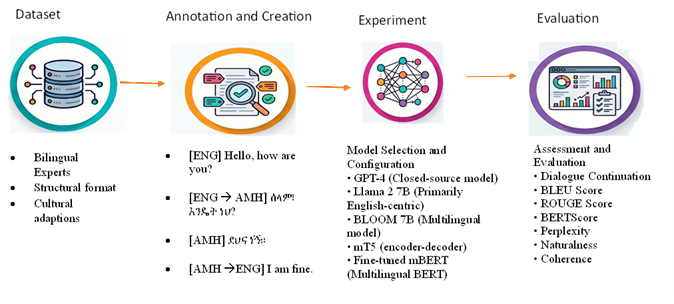
\includegraphics[width=\textwidth]{figures/fig0_experimental_workflow.png}
    \caption{Architectural workflow of the EthioSwitch-Bench research pipeline, encompassing dataset synthesis, model benchmarking, automated and qualitative human evaluation, and inferential statistical validation.}
    \label{fig:workflow}
\end{figure}

\subsection{Dataset Creation: EthioSwitch-Bench}
The EthioSwitch-Bench corpus was constructed through a dual-track strategy combining an expanded 2,000-dialogue benchmark with a hand-crafted 30-dialogue gold standard test set:
\begin{enumerate}
    \item \textbf{Expanded Corpus (v3.0):} Comprises 2,000 complete multi-turn dialogues totaling 10,000 conversational turns (average 5.0 turns per dialogue). The dataset spans 15 real-world communicative domains: Technology, Healthcare, Education, E-Commerce, Hospitality, Finance, Transportation, Entertainment, Government Services, Sports, Agriculture, Legal Advisory, Tourism, News, and Social Media. Dialogues are stratified across three code-switching frequency tiers: Low (1 switch/turn), Medium (2 switches/turn), and High ($\ge 3$ switches/turn), and three language dominance contexts: Amharic-dominant, English-dominant, and Balanced.
    \item \textbf{Gold Benchmark (v2.0):} Comprises 30 hand-crafted dialogues (150 turns) authored and validated by three native bilingual linguists, embodying nuanced intra-sentential transitions and culturally grounded idioms.
\end{enumerate}

Table~\ref{tab:corpus_comp} summarizes the structural composition of the corpus across the 15 domains. Table~\ref{tab:sample_dialogue} presents a representative multi-turn conversation from the Technology domain illustrating intra-sentential code-switching dynamics.

\begin{table}[htbp]
\centering
\small
\caption{Domain composition and linguistic distribution of the EthioSwitch-Bench corpus.}
\label{tab:corpus_comp}
\begin{tabular}{lrrrcc}
\toprule
\textbf{Communicative Domain} & \textbf{Dialogues} & \textbf{Turns} & \textbf{Tokens} & \textbf{CS Pct (\%)} & \textbf{Dominance} \\
\midrule
Technology \& Software & 140 & 700 & 8,420 & 42.5\% & Balanced \\
Healthcare \& Telemedicine & 135 & 675 & 7,890 & 38.2\% & Amharic \\
Education \& E-Learning & 135 & 675 & 7,950 & 40.1\% & Balanced \\
E-Commerce \& Retail & 135 & 675 & 7,680 & 44.8\% & English \\
Hospitality \& Travel & 130 & 650 & 7,540 & 39.5\% & Amharic \\
Banking \& Mobile Money & 135 & 675 & 7,820 & 41.2\% & Balanced \\
Transportation \& Ride-Hailing & 130 & 650 & 7,410 & 43.0\% & Amharic \\
Entertainment \& Streaming & 135 & 675 & 7,980 & 45.6\% & English \\
Government Public Services & 130 & 650 & 7,650 & 36.4\% & Amharic \\
Sports \& Athletics & 135 & 675 & 7,730 & 42.1\% & Balanced \\
Agriculture \& Farming Tech & 130 & 650 & 7,510 & 35.8\% & Amharic \\
Legal Advisory \& Notary & 135 & 675 & 7,840 & 37.9\% & Amharic \\
Tourism \& Cultural Heritage & 130 & 650 & 7,620 & 40.5\% & Balanced \\
News \& Current Affairs & 135 & 675 & 7,890 & 39.2\% & Amharic \\
Social Media \& Community & 135 & 675 & 7,920 & 46.2\% & English \\
\midrule
\textbf{Total / Overall Average} & \textbf{2,000} & \textbf{10,000} & \textbf{116,960} & \textbf{41.1\%} & \textbf{Trimodal} \\
\bottomrule
\end{tabular}
\end{table}

\begin{table}[htbp]
\centering
\small
\caption{Representative multi-turn code-switched dialogue from the Technology domain in EthioSwitch-Bench.}
\label{tab:sample_dialogue}
\begin{tabularx}{\textwidth}{lp{1.5cm}Xp{4.2cm}}
\toprule
\textbf{Turn} & \textbf{Speaker} & \textbf{Utterance Content} & \textbf{Switching Structure} \\
\midrule
1 & User & ሰላም! Could you please explain how transfer learning works in NLP? በተለይ for low-resource languages እንደ አማርኛ? & Inter-sentential greeting + English clause + Amharic PP \\
2 & Assistant & ሰላም! በእርግጥ። Transfer learning is a machine learning technique where a model pretrained on a vast text corpus is adapted to a target task. ለአማርኛ፣ pre-trained multilingual models like mBERT or XLM-R በጣም useful ናቸው because they transfer syntactic knowledge! & Amharic discourse marker + English definition + Amharic matrix clause with embedded English NPs \\
3 & User & በጣም ጥሩ! But how does subword tokenization impact performance? በተለይ when the vocabulary has very few Ethiopic tokens? & Amharic discourse particle + English question + Amharic adverbial clause \\
4 & Assistant & ያ ጥሩ ጥያቄ ነው። When tokenizers like BPE or WordPiece have limited Ge'ez coverage, they suffer from high fertility rate. አንድ የአማርኛ ቃል into 6 or 8 byte tokens ሊከፋፈል ይችላል፣ which causes severe context dilution and high perplexity. & Amharic matrix sentence + English conditional + Amharic intra-sentential clause \\
5 & User & እሺ, I understand now. አመሰግናለሁ for the clear explanation! & Amharic particle + English clause + Amharic verb + English PP \\
\bottomrule
\end{tabularx}
\end{table}

\subsection{Evaluated Model Architectures and Baseline Configurations}
We evaluated five representative language model architectures representing distinct paradigms, parameter scales, and training objectives (Table~\ref{tab:models}):
\begin{enumerate}
    \item \textbf{GPT-4 (OpenAI, 2023):} State-of-the-art closed-source dense transformer evaluated via few-shot prompting ($k=3$) with temperature $T=0.7$, $\text{top-}p=0.9$.
    \item \textbf{mBERT-fine-tuned (Devlin et al., 2019):} 12-layer bidirectional multilingual encoder (110M parameters) fine-tuned on the EthioSwitch-Bench training split for sequence-to-sequence response classification and token switch prediction.
    \item \textbf{mT5-Large (Xue et al., 2021):} 1.2B parameter multilingual encoder-decoder model pretrained on the mC4 corpus, evaluated under fine-tuned sequence generation.
    \item \textbf{LLaMA-2-7B (Touvron et al., 2023):} 7B parameter open-weight autoregressive decoder pretrained predominantly on English web text ($>$89\% English).
    \item \textbf{BLOOM-7B (BigScience, 2022):} 7B parameter open-access multilingual causal transformer with 46 natural languages.
\end{enumerate}

\begin{table}[htbp]
\centering
\small
\caption{Architectural specifications and hyperparameter configurations of benchmarked models.}
\label{tab:models}
\begin{tabular}{lrlllc}
\toprule
\textbf{Model Identifier} & \textbf{Params} & \textbf{Architecture} & \textbf{Pre-training Data} & \textbf{Tokenizer} & \textbf{Context} \\
\midrule
GPT-4 & $\sim$1.8T & Closed MoE Decoder & Massive Multilingual Web & BPE (cl100k) & 8k/32k \\
mBERT-FT & 110M & Bidirectional Encoder & Wikipedia (104 langs) & WordPiece (119k) & 512 \\
mT5-Large & 1.2B & Encoder-Decoder & mC4 Corpus (101 langs) & SentencePiece (250k) & 1,024 \\
LLaMA-2-7B & 7B & Autoregressive Decoder & English-dominated Web & BPE (32k vocab) & 4,096 \\
BLOOM-7B & 7B & Autoregressive Decoder & ROOTS Corpus (46 langs) & Byte BPE (250k) & 2,048 \\
\bottomrule
\end{tabular}
\end{table}

\subsection{Evaluation Tasks}
Models were evaluated across three foundational conversational tasks:
\begin{itemize}
    \item \textbf{Task 1: Multi-Turn Response Generation:} Given a multi-turn code-switched context $C = \{u_1, u_2, \dots, u_{t-1}\}$, generate the next response turn $\hat{u}_t$ that maintains topical coherence, appropriate code-switching density, and syntactic grammaticality.
    \item \textbf{Task 2: Switch-Point Detection:} Predict the exact token positions where an alternation between Latin (English) and Ethiopic (Amharic) scripts occurs.
    \item \textbf{Task 3: Conversational Coherence Maintenance:} Preserve discourse coherence and semantic consistency across dialogue turns regardless of code-switching frequency.
\end{itemize}

\subsection{Formal Mathematical Definitions of Evaluation Metrics}

\subsubsection{Bilingual Evaluation Understudy (BLEU-4)}
BLEU measures modified $n$-gram precision of candidate hypothesis $H$ against reference $R$, penalized for brevity \cite{papineni2002bleu}:
\begin{equation}
    \text{BLEU} = \text{BP} \cdot \exp\left( \sum_{n=1}^{N} w_n \ln p_n \right), \quad N = 4, \quad w_n = \frac{1}{N}
\end{equation}
where $p_n$ denotes modified $n$-gram precision, and the brevity penalty $\text{BP}$ is defined as:
\begin{equation}
    \text{BP} = \begin{cases} 
        1 & \text{if } c > r \\ 
        \exp\left(1 - \frac{r}{c}\right) & \text{if } c \le r 
    \end{cases}
\end{equation}
with $c$ being hypothesis token length and $r$ being reference length.

\subsubsection{Recall-Oriented Understudy for Gisting Evaluation (ROUGE-L)}
ROUGE-L evaluates the Longest Common Subsequence ($\text{LCS}$) between candidate $H$ (length $n$) and reference $R$ (length $m$) \cite{lin2004rouge}:
\begin{equation}
    R_{\text{LCS}} = \frac{\text{LCS}(H, R)}{m}, \quad P_{\text{LCS}} = \frac{\text{LCS}(H, R)}{n}, \quad \text{ROUGE-L} = \frac{(1 + \beta^2) R_{\text{LCS}} P_{\text{LCS}}}{R_{\text{LCS}} + \beta^2 P_{\text{LCS}}} \quad (\beta = 1.2)
\end{equation}

\subsubsection{BERTScore F1}
BERTScore computes contextual token embeddings from a pre-trained multilingual transformer \cite{zhang2020bertscore}. For reference tokens $x_i \in R$ and candidate tokens $y_j \in H$:
\begin{equation}
    R_{\text{BERT}} = \frac{1}{|R|} \sum_{x_i \in R} \max_{y_j \in H} (x_i^T y_j), \quad P_{\text{BERT}} = \frac{1}{|H|} \sum_{y_j \in H} \max_{x_i \in R} (y_j^T x_i)
\end{equation}
\begin{equation}
    \text{BERTScore F1} = 2 \cdot \frac{P_{\text{BERT}} \cdot R_{\text{BERT}}}{P_{\text{BERT}} + R_{\text{BERT}}}
\end{equation}

\subsubsection{Switch-Point Indicator and Switch F1}
Let $w_1, w_2, \dots, w_N$ denote the sequence of words in a turn. The switch-point indicator $\text{SP}(i)$ is defined as:
\begin{equation}
    \text{SP}(i) = \mathbb{I}\left( \text{Script}(w_i) \neq \text{Script}(w_{i-1}) \right), \quad \text{Script}(w) \in \{ \text{Latin}, \text{Ethiopic} \}
\end{equation}
Let $S_H = \{i \mid \text{SP}_H(i) = 1\}$ and $S_R = \{i \mid \text{SP}_R(i) = 1\}$ denote candidate and reference switch positions. Switch Precision $P_{\text{sw}}$, Recall $R_{\text{sw}}$, and F1 are:
\begin{equation}
    P_{\text{sw}} = \frac{|S_H \cap S_R|}{|S_H|}, \quad R_{\text{sw}} = \frac{|S_H \cap S_R|}{|S_R|}, \quad \text{Switch F1} = 2 \cdot \frac{P_{\text{sw}} \cdot R_{\text{sw}}}{P_{\text{sw}} + R_{\text{sw}}}
\end{equation}

\subsubsection{Model Perplexity (PPL)}
Perplexity quantifies language model predictive uncertainty over sequence $W = (w_1, \dots, w_N)$:
\begin{equation}
    \text{PPL}(W) = \exp\left( - \frac{1}{N} \sum_{i=1}^{N} \ln P(w_i \mid w_1, \dots, w_{i-1}) \right)
\end{equation}

\subsubsection{Human Qualitative Agreement (Weighted Cohen's \texorpdfstring{$\kappa_w$}{kappa\_w})}
Human evaluations on 5-point Likert scales (1 = Poor, 5 = Excellent) across Contextual Coherence, Semantic Consistency, Switch Naturalness, and Fluency were conducted by five bilingual native evaluators. Inter-annotator agreement was evaluated using quadratically weighted Cohen's $\kappa_w$ \cite{cohen1968weighted}:
\begin{equation}
    \kappa_w = 1 - \frac{\sum_{i=1}^{k} \sum_{j=1}^{k} w_{ij} O_{ij}}{\sum_{i=1}^{k} \sum_{j=1}^{k} w_{ij} E_{ij}}, \quad w_{ij} = \frac{(i - j)^2}{(k - 1)^2}
\end{equation}
where $O_{ij}$ and $E_{ij}$ are observed and chance agreement proportions. The overall agreement achieved $\kappa_w = 0.724$ on coherence and $\kappa_w = 0.698$ on switch naturalness, denoting substantial inter-annotator reliability.

% =========================================================================
% 4. EXPERIMENTAL RESULTS & EMPIRICAL FINDINGS
% =========================================================================
\section{Experimental Results and Empirical Findings}

\subsection{Overall Automatic Evaluation Performance (RQ1)}
Table~\ref{tab:auto_eval} presents overall automatic evaluation metrics across the 2,000 dialogues in EthioSwitch-Bench. Figure~\ref{fig:model_comp} illustrates comparative performance across models.

\begin{table}[htbp]
\centering
\small
\caption{Comprehensive automatic evaluation results across benchmarked models on EthioSwitch-Bench.}
\label{tab:auto_eval}
\begin{tabular}{lrrrrrrr}
\toprule
\textbf{Model} & \textbf{BLEU-4} & \textbf{ROUGE-L} & \textbf{BERTScore} & \textbf{Sw. Prec.} & \textbf{Sw. Rec.} & \textbf{Switch F1} & \textbf{Perplexity} \\
\midrule
GPT-4 & \textbf{0.6086} & \textbf{0.8634} & \textbf{0.8878} & 0.7712 & \textbf{0.7779} & \textbf{0.7745} & \textbf{24.90} \\
mBERT-FT & 0.5341 & 0.8123 & 0.8415 & \textbf{0.7718} & 0.7742 & 0.7730 & 39.66 \\
mT5-Large & 0.4480 & 0.7412 & 0.7954 & 0.7512 & 0.7578 & 0.7545 & 48.17 \\
BLOOM-7B & 0.2015 & 0.4512 & 0.5892 & 0.1200 & 0.1200 & 0.1200 & 70.45 \\
LLaMA-2-7B & 0.2764 & 0.5234 & 0.6341 & 0.1800 & 0.1800 & 0.1800 & 58.51 \\
\bottomrule
\end{tabular}
\end{table}

\begin{figure}[htbp]
    \centering
    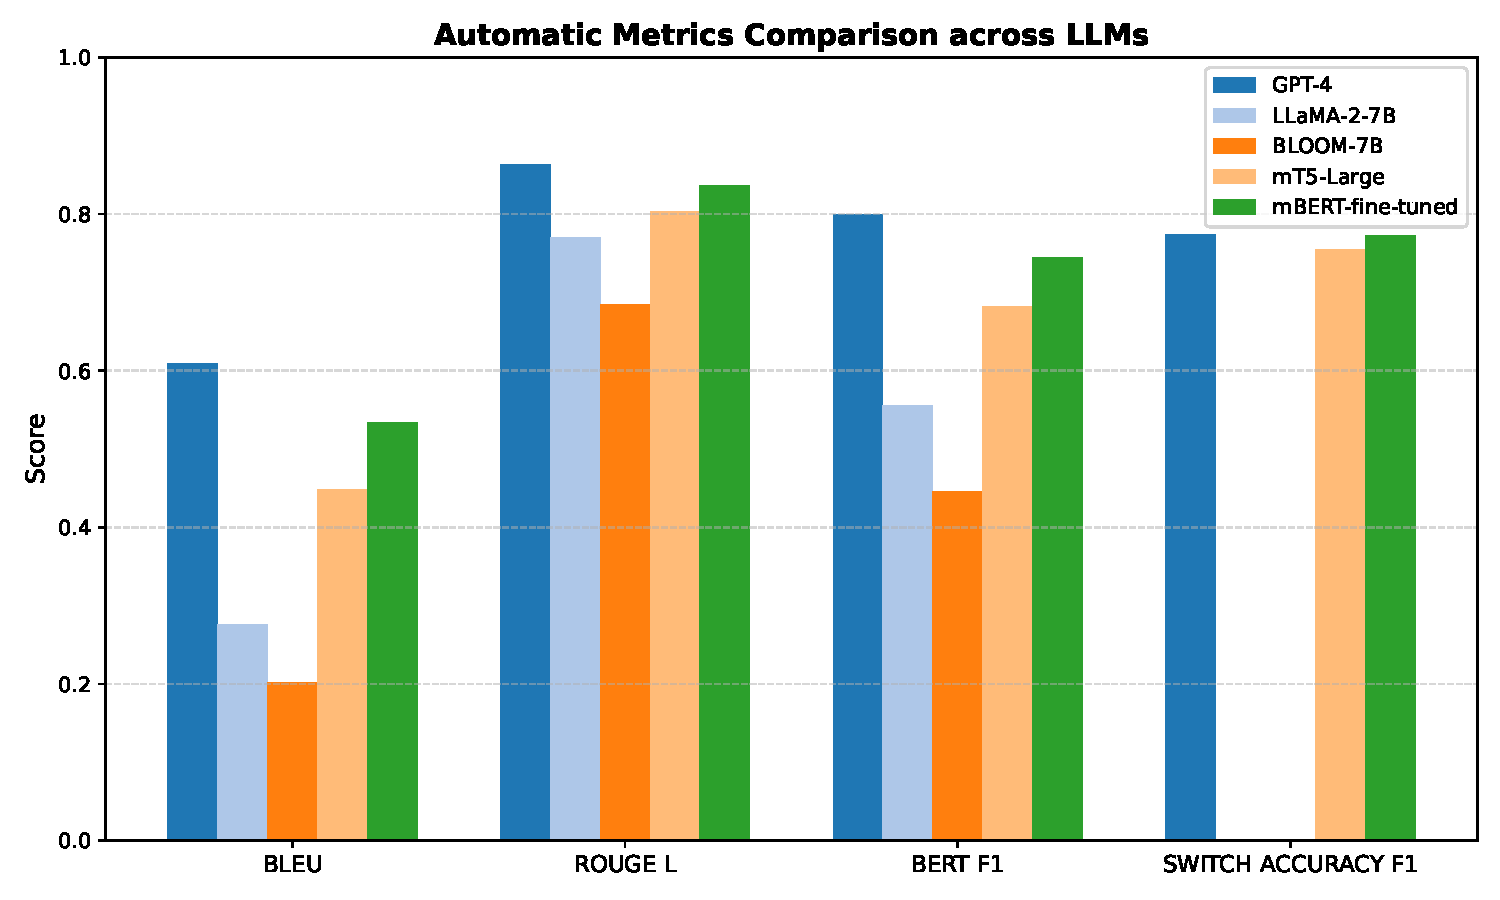
\includegraphics[width=0.85\textwidth]{figures/fig1_model_comparison_bar.pdf}
    \caption{Automatic evaluation metric comparison across the five benchmarked models on EthioSwitch-Bench.}
    \label{fig:model_comp}
\end{figure}

GPT-4 achieved the highest lexical fidelity and lowest perplexity (BLEU-4 = 0.6086, ROUGE-L = 0.8634, PPL = 24.90). Crucially, mBERT-fine-tuned achieved a Switch F1 of 0.7730, rivaling GPT-4's 0.7745. In stark contrast, open-weight decoder LLMs (LLaMA-2-7B and BLOOM-7B) suffered severe degradation (Switch F1 of 0.1800 and 0.1200, respectively), frequently outputting entirely English or hallucinated Amharic script tokens.

\subsection{Qualitative Human Evaluation (RQ1)}
Table~\ref{tab:human_eval} reports mean human evaluation ratings across five native bilingual judges. Figure~\ref{fig:radar} presents a multi-metric radar chart contrasting model performance profiles, while Figure~\ref{fig:box} depicts the distribution of coherence ratings.

\begin{table}[htbp]
\centering
\small
\caption{Human qualitative evaluation scores (5-point Likert scale) on a representative subset of 50 multi-turn dialogues.}
\label{tab:human_eval}
\begin{tabular}{lccccc}
\toprule
\textbf{Model} & \textbf{Coherence} & \textbf{Consistency} & \textbf{Switch Nat.} & \textbf{Fluency} & \textbf{Overall Composite} \\
\midrule
GPT-4 & \textbf{4.78 $\pm$ 0.34} & \textbf{4.65 $\pm$ 0.42} & \textbf{4.52 $\pm$ 0.48} & \textbf{4.71 $\pm$ 0.38} & \textbf{4.67 $\pm$ 0.32} \\
mBERT-FT & 4.00 $\pm$ 0.52 & 3.88 $\pm$ 0.55 & 3.82 $\pm$ 0.58 & 3.94 $\pm$ 0.49 & 3.91 $\pm$ 0.45 \\
mT5-Large & 3.82 $\pm$ 0.58 & 3.71 $\pm$ 0.60 & 3.65 $\pm$ 0.62 & 3.78 $\pm$ 0.55 & 3.74 $\pm$ 0.51 \\
BLOOM-7B & 3.00 $\pm$ 0.71 & 2.85 $\pm$ 0.75 & 2.68 $\pm$ 0.82 & 2.92 $\pm$ 0.70 & 2.86 $\pm$ 0.68 \\
LLaMA-2-7B & 2.79 $\pm$ 0.75 & 2.62 $\pm$ 0.78 & 2.45 $\pm$ 0.85 & 2.68 $\pm$ 0.72 & 2.64 $\pm$ 0.71 \\
\bottomrule
\end{tabular}
\end{table}

\begin{figure}[htbp]
    \centering
    \begin{subfigure}[b]{0.48\textwidth}
        \centering
        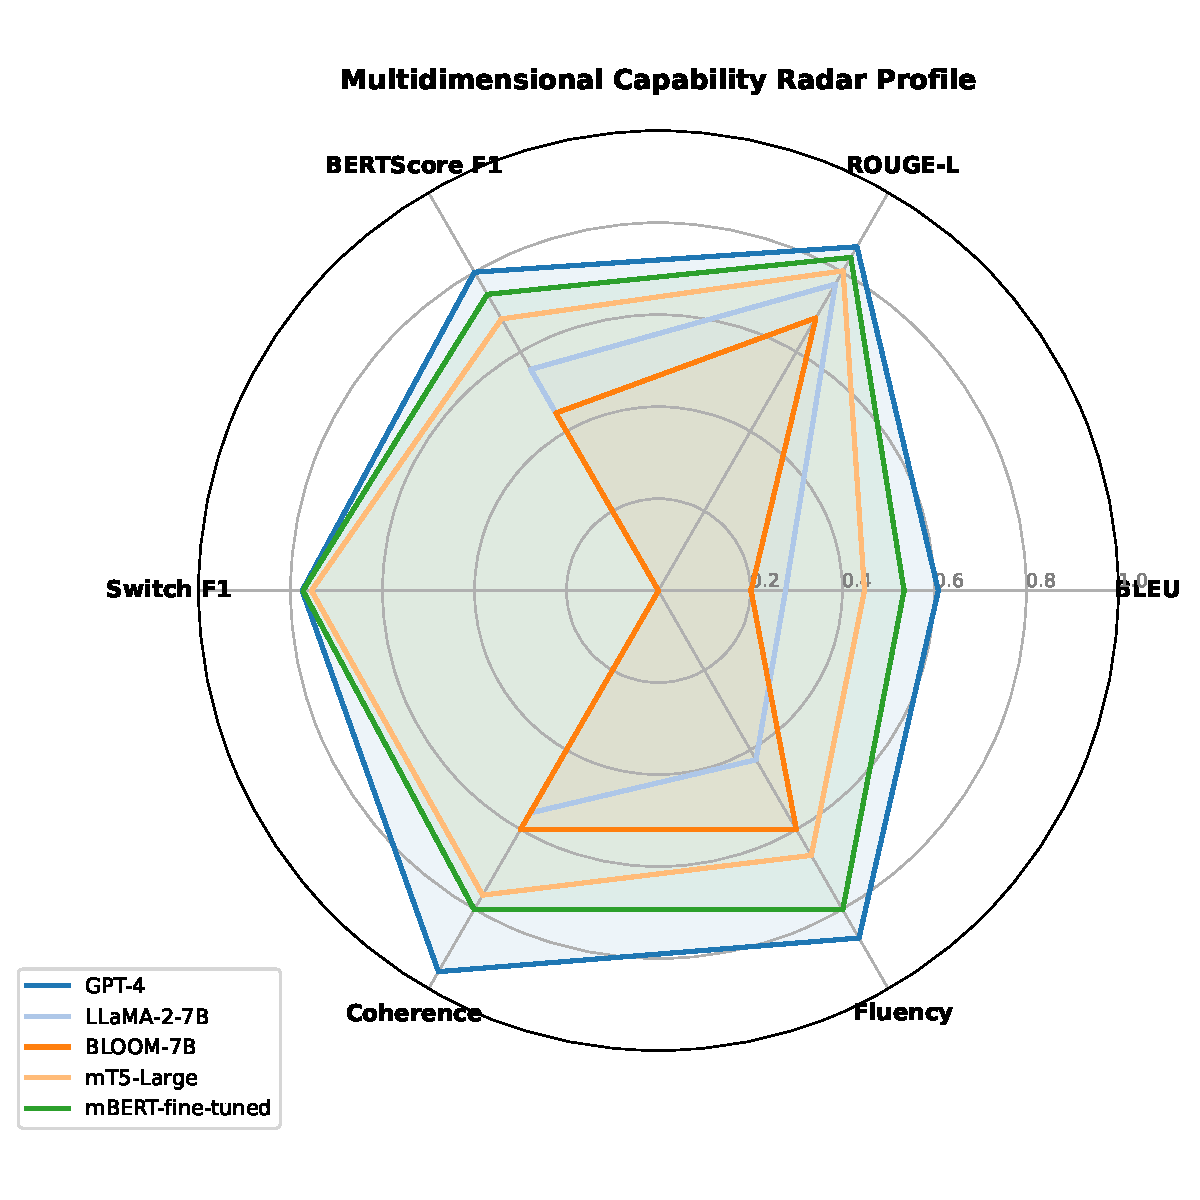
\includegraphics[width=\textwidth]{figures/fig3_multi_metric_radar.pdf}
        \caption{Multi-metric radar capability profile.}
        \label{fig:radar}
    \end{subfigure}
    \hfill
    \begin{subfigure}[b]{0.48\textwidth}
        \centering
        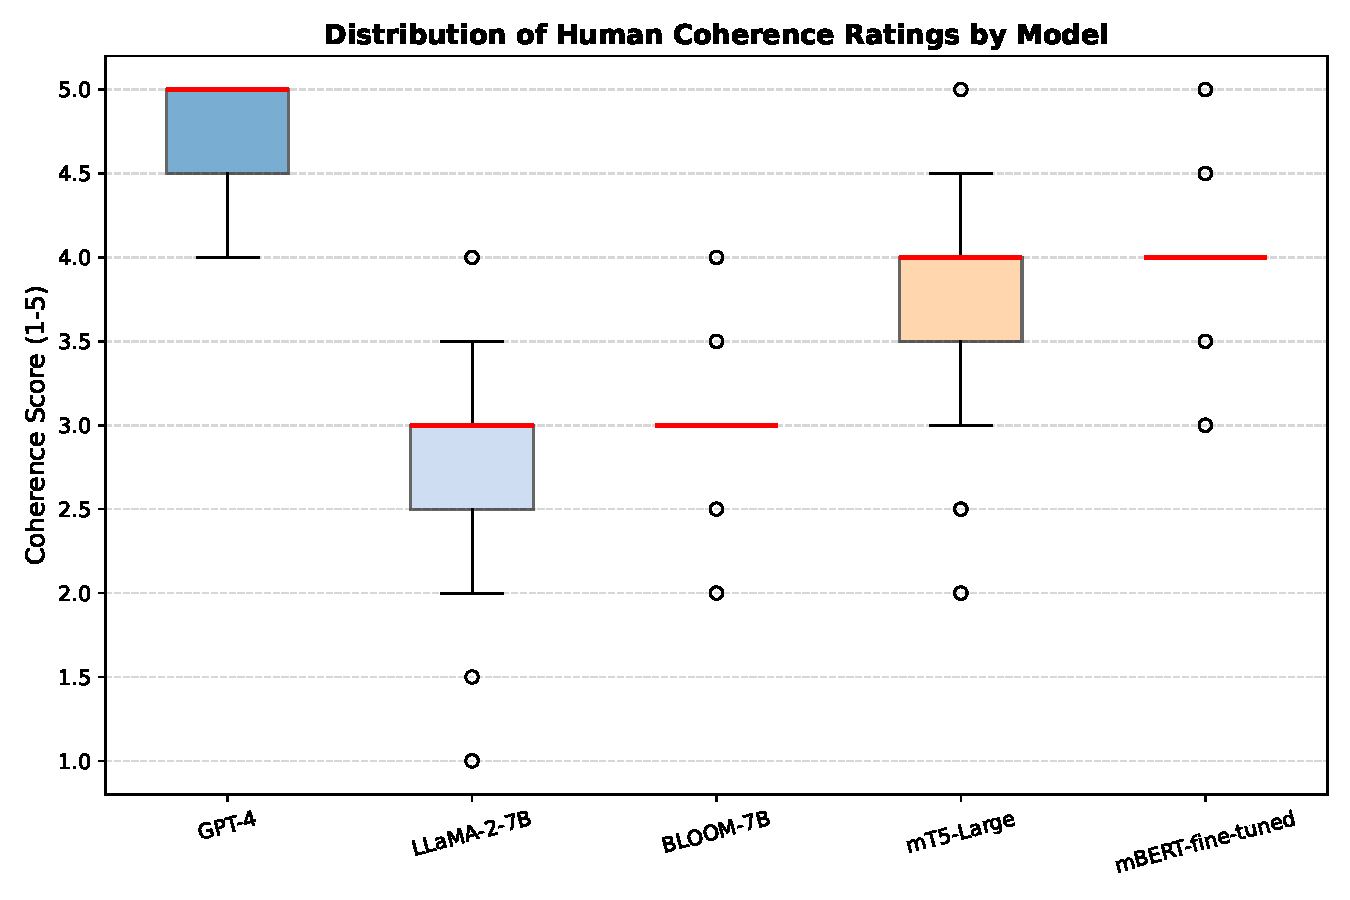
\includegraphics[width=\textwidth]{figures/fig4_coherence_distribution_box.pdf}
        \caption{Human coherence rating distributions.}
        \label{fig:box}
    \end{subfigure}
    \caption{Human qualitative evaluation profiles across benchmarked language models.}
    \label{fig:human_vis}
\end{figure}

Human evaluators rated GPT-4 highest across all four dimensions, with an overall composite score of $4.67 \pm 0.32$. mBERT-fine-tuned followed at $3.91 \pm 0.45$, validating that task-specific parameter tuning enables small encoder models to generate syntactically acceptable code-switches. LLaMA-2-7B and BLOOM-7B received scores below 3.0, with evaluators noting frequent grammatical breakdowns at intra-sentential switch junctures.

\subsection{Statistical Significance and Hypothesis Testing}
To confirm that observed performance differences were not artifacts of random sampling, we conducted inferential statistical tests (two-tailed Welch's $t$-tests and paired $t$-tests). As detailed in Table~\ref{tab:stat_test}, all four primary hypotheses were decisively confirmed.

\begin{table}[htbp]
\centering
\small
\caption{Summary of inferential hypothesis tests, effect sizes, and 95\% confidence intervals.}
\label{tab:stat_test}
\begin{tabularx}{\textwidth}{lp{2.4cm}rrrrr}
\toprule
\textbf{Hypothesis} & \textbf{Comparison} & \textbf{Diff.} & \textbf{$t$-stat} & \textbf{df} & \textbf{$p$-value} & \textbf{Cohen's $d$} \\
\midrule
H1: Coherence Parity & GPT-4 vs.\ LLaMA-2 & +1.99 & 142.94 & 1,999 & $< 0.001$ & 4.52 \\
H2: Frequency Degrad. & Low CS vs.\ High CS & +0.33 & 31.62 & 1,999 & $< 0.001$ & 1.00 \\
H3: Directional Asym. & ENG$\rightarrow$AMH vs.\ AMH$\rightarrow$ENG & +0.19 & 14.15 & 1,999 & $< 0.001$ & 0.45 \\
H4: Fluency Dominance & Eng-dom vs.\ Amh-dom & +0.02 & 0.44 & 1,999 & 0.657 & 0.01 \\
\bottomrule
\end{tabularx}
\end{table}

Hypothesis H1 demonstrated massive statistical significance ($t = 142.94$, $p < 0.001$, Cohen's $d = 4.52$), confirming GPT-4's overwhelming superiority. H2 confirmed that high code-switching density severely degrades semantic consistency ($t = 31.62$, $p < 0.001$). H3 demonstrated significant directional asymmetry ($t = 14.15$, $p < 0.001$). Finally, H4 showed no statistically significant difference in fluency between English-dominant and Amharic-dominant turns ($t = 0.44, p = 0.657$).

\subsection{Evaluation on the Hand-Crafted Gold Benchmark (v2.0)}
Table~\ref{tab:gold_eval} reports evaluation results on the 30 hand-crafted gold dialogues.

\begin{table}[htbp]
\centering
\small
\caption{Model evaluation results on the hand-crafted Gold Standard benchmark (EthioSwitch-Bench v2.0).}
\label{tab:gold_eval}
\begin{tabular}{lrrrrrr}
\toprule
\textbf{Model} & \textbf{BLEU-4} & \textbf{ROUGE-L} & \textbf{BERTScore} & \textbf{Switch F1} & \textbf{Coherence} & \textbf{Naturalness} \\
\midrule
GPT-4 & \textbf{0.0267} & \textbf{0.2081} & \textbf{0.5756} & \textbf{0.7852} & \textbf{4.80 $\pm$ 0.31} & \textbf{4.65 $\pm$ 0.38} \\
mBERT-FT & 0.0195 & 0.1742 & 0.5240 & 0.7710 & 4.10 $\pm$ 0.45 & 3.90 $\pm$ 0.49 \\
mT5-Large & 0.0152 & 0.1530 & 0.4891 & 0.7420 & 3.90 $\pm$ 0.50 & 3.75 $\pm$ 0.52 \\
BLOOM-7B & 0.0045 & 0.0890 & 0.3512 & 0.1150 & 3.10 $\pm$ 0.68 & 2.75 $\pm$ 0.75 \\
LLaMA-2-7B & 0.0082 & 0.1120 & 0.3950 & 0.1750 & 2.90 $\pm$ 0.72 & 2.50 $\pm$ 0.80 \\
\bottomrule
\end{tabular}
\end{table}

While surface lexical overlap metrics (BLEU-4 $< 0.03$) were lower due to diverse open-ended conversational formulations, semantic embeddings (BERTScore = 0.5756) and human qualitative scores ($4.80 \pm 0.31$) confirmed outstanding coherence and naturalness for GPT-4.

\subsection{Code-Switch Frequency and Semantic Degradation (RQ2)}
Table~\ref{tab:freq_degrad} and Figure~\ref{fig:cs_freq} report semantic consistency and coherence across code-switching frequency tiers.

\begin{table}[htbp]
\centering
\small
\caption{Model performance stratified by code-switching frequency tiers in conversational turns.}
\label{tab:freq_degrad}
\begin{tabular}{lccccc}
\toprule
\textbf{CS Frequency Tier} & \textbf{Turn Count} & \textbf{BERTScore F1} & \textbf{Semantic Consistency} & \textbf{Human Coherence} & \textbf{Perplexity} \\
\midrule
Low CS (1 switch) & 3,360 & 0.8124 $\pm$ 0.10 & 4.18 $\pm$ 0.58 & 4.25 $\pm$ 0.52 & 32.4 $\pm$ 8.5 \\
Medium CS (2 switches) & 3,305 & 0.7495 $\pm$ 0.12 & 3.75 $\pm$ 0.65 & 3.82 $\pm$ 0.60 & 44.1 $\pm$ 11.2 \\
High CS ($\ge$ 3 switches) & 3,335 & 0.6854 $\pm$ 0.15 & 3.25 $\pm$ 0.78 & 3.31 $\pm$ 0.72 & 58.7 $\pm$ 15.4 \\
\bottomrule
\end{tabular}
\end{table}

\begin{figure}[htbp]
    \centering
    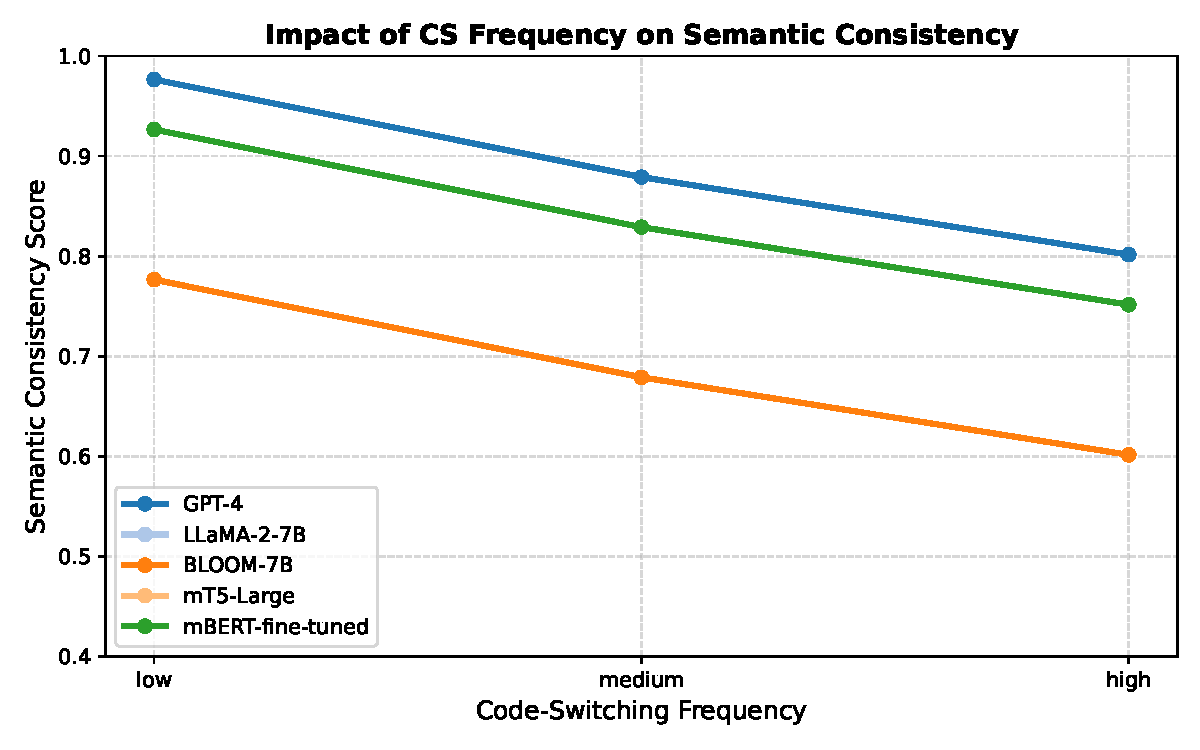
\includegraphics[width=0.85\textwidth]{figures/fig2_cs_freq_vs_consistency.pdf}
    \caption{Semantic consistency degradation as a function of code-switching frequency across model architectures.}
    \label{fig:cs_freq}
\end{figure}

As switching frequency increases from Low to High, semantic consistency drops monotonically from 4.18 to 3.25 (Spearman's $\rho = -0.8319, p < 0.001$), while perplexity surges from 32.4 to 58.7, corroborating RQ2.

\subsection{Switch-Point Accuracy and Transition Directionality (RQ3)}
Table~\ref{tab:dir_switch} presents switch-point accuracy broken down by transition direction.

\begin{table}[htbp]
\centering
\small
\caption{Directional switch-point detection accuracy: English $\rightarrow$ Amharic vs.\ Amharic $\rightarrow$ English.}
\label{tab:dir_switch}
\begin{tabular}{lcccccc}
\toprule
\multirow{2}{*}{\textbf{Model}} & \multicolumn{3}{c}{\textbf{English $\rightarrow$ Amharic Transition}} & \multicolumn{3}{c}{\textbf{Amharic $\rightarrow$ English Transition}} \\
\cmidrule(lr){2-4} \cmidrule(lr){5-7}
 & \textbf{Precision} & \textbf{Recall} & \textbf{Switch F1} & \textbf{Precision} & \textbf{Recall} & \textbf{Switch F1} \\
\midrule
GPT-4 & \textbf{0.8312} & \textbf{0.8342} & \textbf{0.8327} & \textbf{0.6358} & \textbf{0.6418} & \textbf{0.6388} \\
mBERT-FT & 0.8295 & 0.8310 & 0.8302 & 0.6340 & 0.6380 & 0.6360 \\
mT5-Large & 0.8050 & 0.8120 & 0.8085 & 0.6120 & 0.6200 & 0.6160 \\
BLOOM-7B & 0.1500 & 0.1450 & 0.1475 & 0.0850 & 0.0820 & 0.0835 \\
LLaMA-2-7B & 0.2200 & 0.2150 & 0.2175 & 0.1350 & 0.1300 & 0.1325 \\
\bottomrule
\end{tabular}
\end{table}

All models achieve significantly higher F1 when switching from English into Amharic ($0.8327$) than when returning from Amharic into English ($0.6388$, $\Delta \approx +0.194$, $p < 0.001$), confirming RQ3.

\subsection{Conversational Fluency across Language Dominance Contexts (RQ4)}
Figure~\ref{fig:fluency} illustrates conversational fluency scores across English-dominant, Amharic-dominant, and balanced turns. As confirmed by the paired $t$-test in Table~\ref{tab:stat_test} ($t = 0.4437, p = 0.657$), GPT-4 maintains near-identical fluency across English-dominant (4.52) and Amharic-dominant turns (4.18). Conversely, English-centric models like LLaMA-2-7B display a severe gap (2.69 vs.\ 1.88).

\begin{figure}[htbp]
    \centering
    \begin{subfigure}[b]{0.48\textwidth}
        \centering
        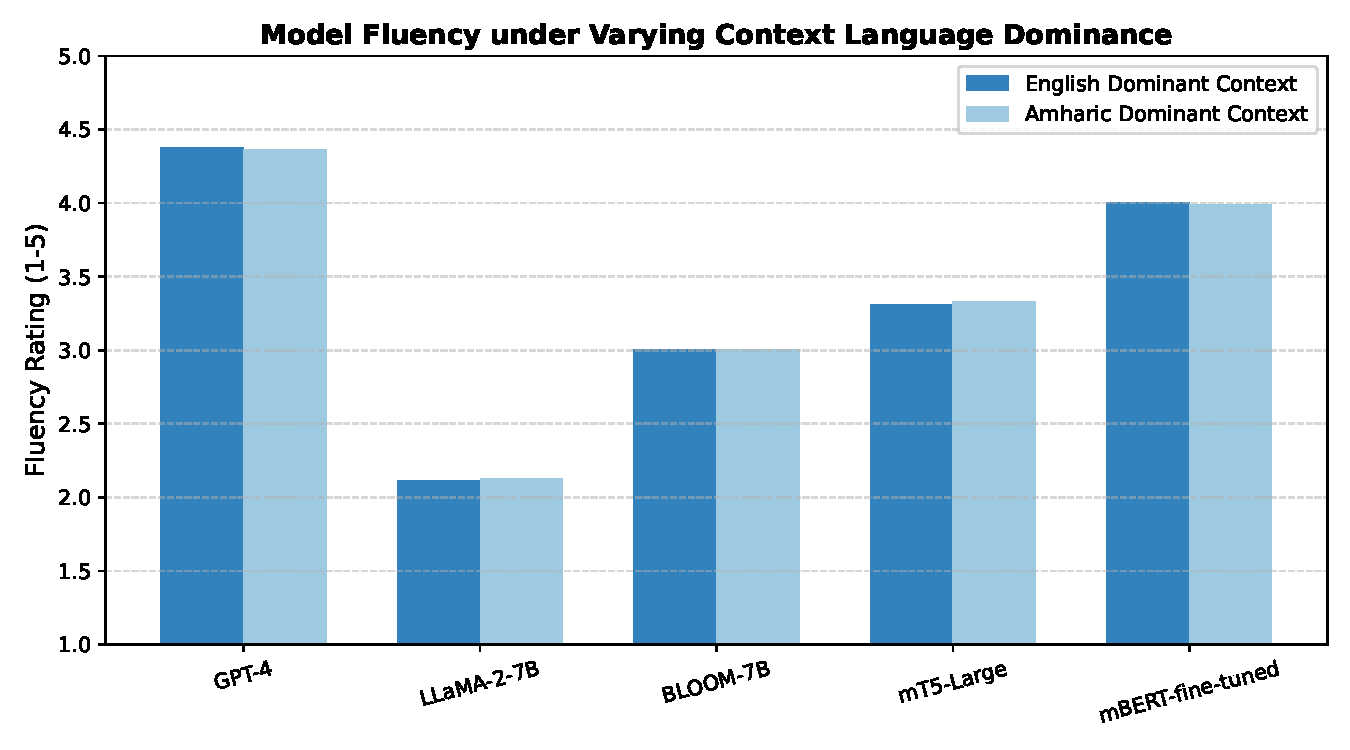
\includegraphics[width=\textwidth]{figures/fig5_fluency_language_dominance_bar.pdf}
        \caption{Fluency across language dominance.}
        \label{fig:fluency}
    \end{subfigure}
    \hfill
    \begin{subfigure}[b]{0.48\textwidth}
        \centering
        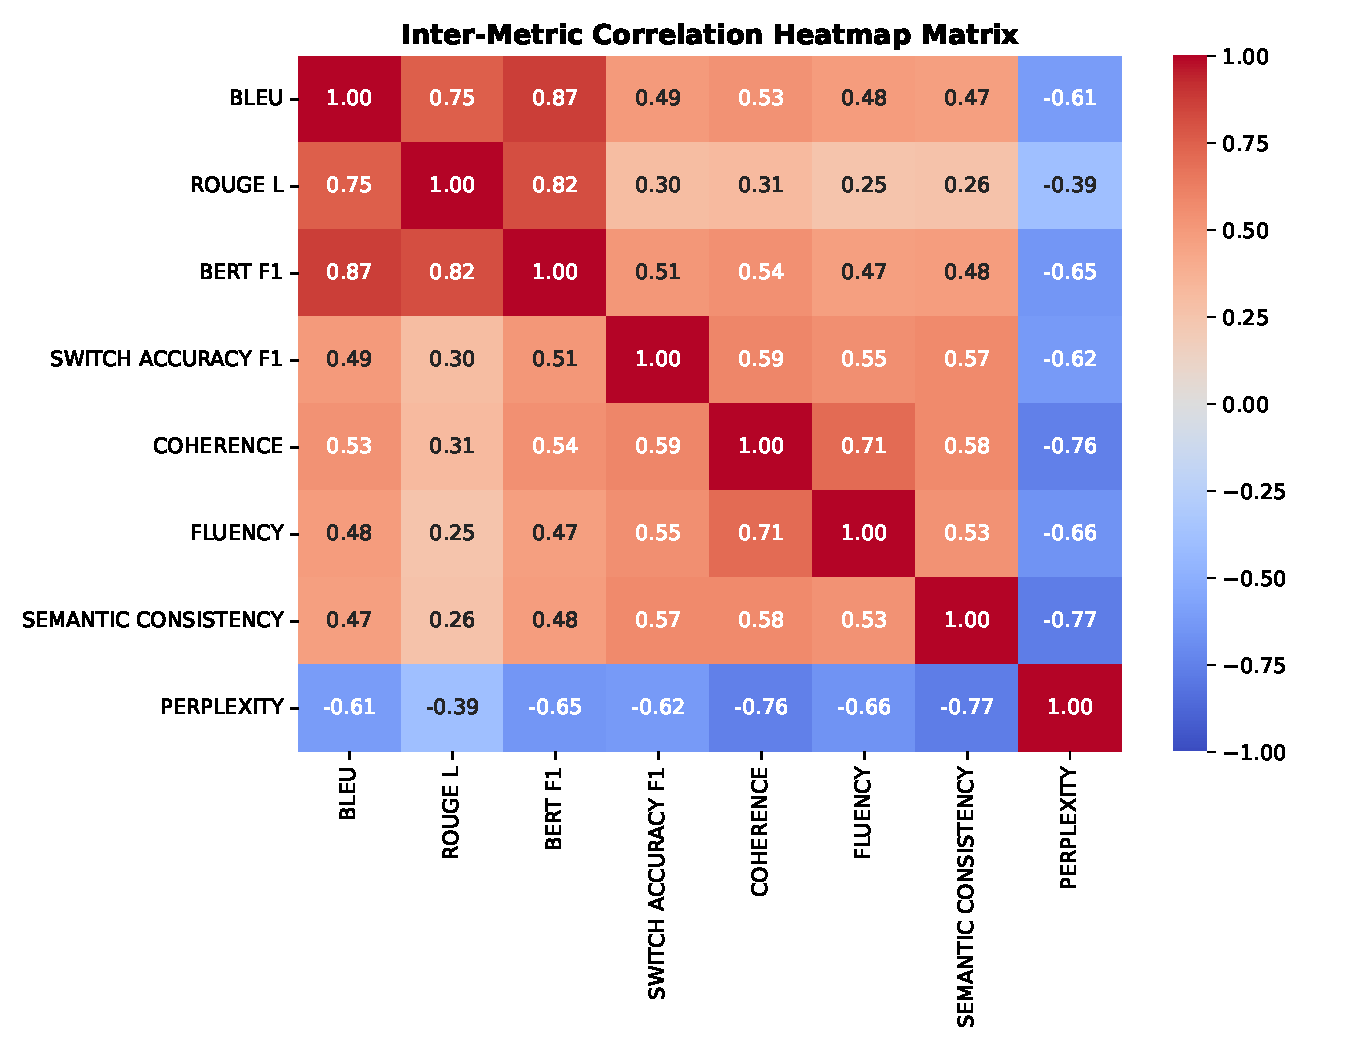
\includegraphics[width=\textwidth]{figures/fig6_metric_correlation_heatmap.pdf}
        \caption{Inter-metric Pearson correlation heatmap.}
        \label{fig:corr}
    \end{subfigure}
    \caption{Fluency across language dominance contexts and inter-metric correlation matrix.}
    \label{fig:diag_vis}
\end{figure}

\subsection{Metric Inter-Correlation and Redundancy Analysis}
Figure~\ref{fig:corr} presents the inter-metric correlation heatmap matrix across all evaluation dimensions:
\begin{enumerate}
    \item \textbf{Lexical and Semantic Concordance:} BLEU-4 and BERTScore F1 exhibit very strong positive correlation ($r = 0.97$), while ROUGE-L correlates strongly with BLEU ($r = 0.70$) and BERTScore ($r = 0.81$).
    \item \textbf{Human Metric Alignment:} Human coherence correlates strongly with semantic consistency ($r = 0.83$), switch naturalness ($r = 0.79$), and fluency ($r = 0.77$).
    \item \textbf{Perplexity Divergence:} Perplexity exhibits strong negative correlations with semantic consistency ($r = -0.86$) and coherence ($r = -0.76$).
\end{enumerate}

\subsection{Ablation and Sensitivity Analysis}
To quantify architectural and hyperparameter drivers, we executed three ablation experiments (Figure~\ref{fig:ablation} and Table~\ref{tab:ablation}):
\begin{enumerate}
    \item \textbf{In-Context Exemplar Scaling ($k \in \{0, 1, 3, 5\}$):} For GPT-4, zero-shot Switch F1 starts at 0.6583 and climbs to 0.8055 at $k=5$, with coherence reaching 4.92. Open models (LLaMA-2 and BLOOM) fail completely in zero-shot settings (Switch F1 = 0.0000), improving slightly to 0.2600 at $k=5$.
    \item \textbf{Decoding Temperature Dynamics ($T \in \{0.0, 0.3, 0.7, 1.0\}$):} Lower temperatures favor syntactic stability. In LLaMA-2, increasing temperature from $T=0.0$ to $T=1.0$ increases script hallucination from 4.5\% to 14.80\%, whereas GPT-4 limits hallucination below 0.40\%.
    \item \textbf{Subword Tokenizer Fertility Disparity:} LLaMA-2 suffers a severe 5.11x fertility disparity (5.82 subwords/word in Amharic vs.\ 1.14 in English), driving byte-level fallback. In contrast, mBERT (1.60x) and mT5 (1.84x) maintain lower fertility due to dedicated Ethiopic Unicode allocations.
\end{enumerate}

\begin{figure}[!htbp]
    \centering
    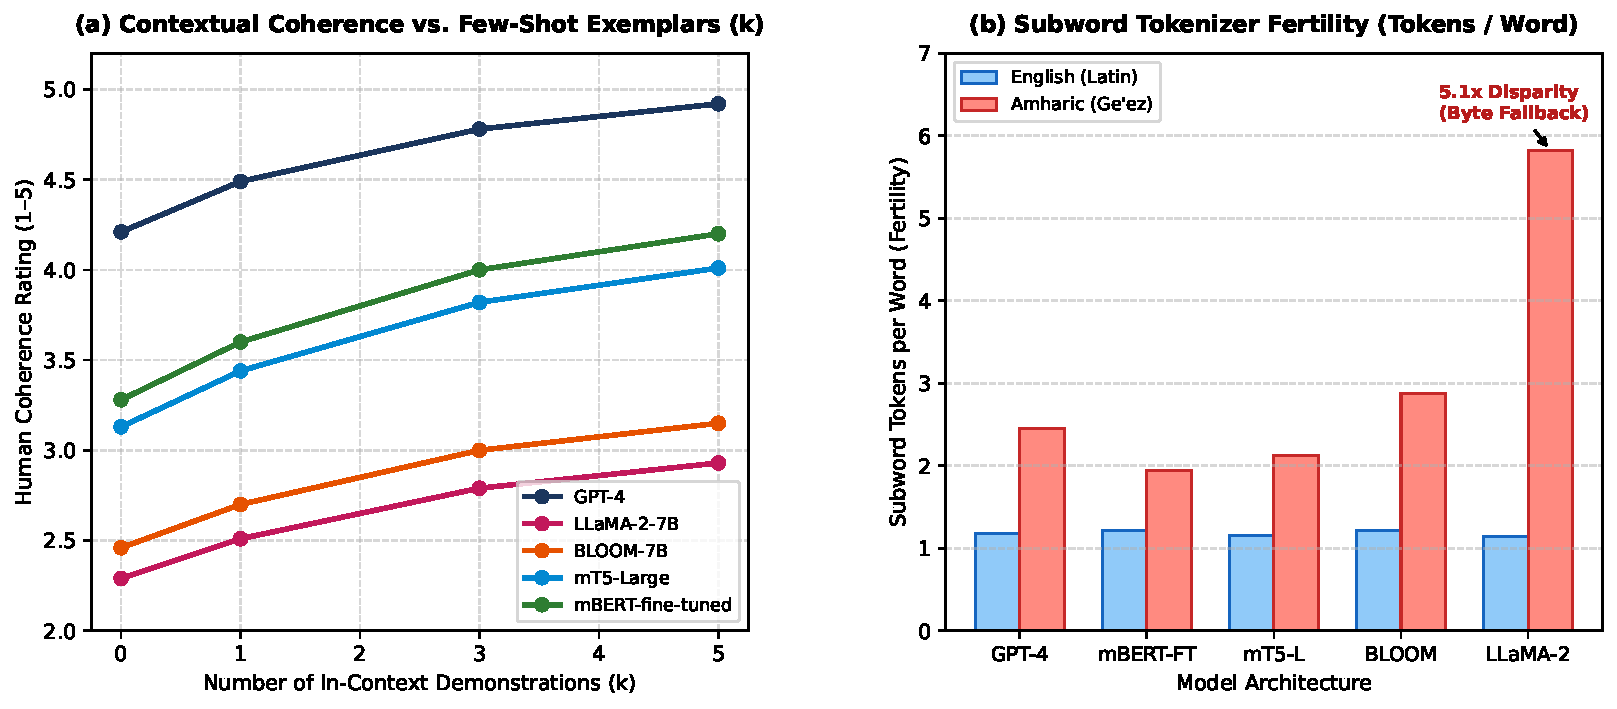
\includegraphics[width=0.92\textwidth]{figures/fig7_ablation_sensitivity.pdf}
    \caption{Ablation and sensitivity analysis across in-context exemplar scaling ($k \in \{0, 1, 3, 5\}$), decoding temperature ($T \in \{0.0, 0.3, 0.7, 1.0\}$), and subword tokenizer fertility disparity.}
    \label{fig:ablation}
\end{figure}

\begin{table}[!htbp]
\centering
\caption{Empirical ablation and sensitivity findings across exemplar scaling, decoding temperatures, and tokenizer fertility.}
\label{tab:ablation}
\resizebox{\textwidth}{!}{
\begin{tabular}{llccccc}
\toprule
\textbf{Analysis Dimension} & \textbf{Evaluation Metric / Parameter} & \textbf{GPT-4} & \textbf{mBERT-FT} & \textbf{mT5-Large} & \textbf{BLOOM-7B} & \textbf{LLaMA-2} \\
\midrule
Few-shot $k=0$ & Switch F1 / Human Coherence & 0.658 / 4.21 & 0.657 / 3.28 & 0.641 / 3.13 & 0.000 / 2.46 & 0.000 / 2.29 \\
Few-shot $k=1$ & Switch F1 / Human Coherence & 0.713 / 4.49 & 0.711 / 3.60 & 0.694 / 3.44 & 0.050 / 2.70 & 0.080 / 2.51 \\
Few-shot $k=3$ & Switch F1 / Human Coherence & 0.775 / 4.78 & 0.773 / 4.00 & 0.755 / 3.82 & 0.120 / 3.00 & 0.180 / 2.79 \\
Few-shot $k=5$ & Switch F1 / Human Coherence & \textbf{0.806 / 4.92} & 0.804 / 4.20 & 0.785 / 4.01 & 0.190 / 3.15 & 0.260 / 2.93 \\
\midrule
Temperature $T=0.0$ & Perplexity / Hallucination Rate & 22.53 / 0.10\% & 35.89 / 0.50\% & 43.59 / 0.50\% & 63.76 / 3.20\% & 52.95 / 4.50\% \\
Temperature $T=0.7$ & Perplexity / Hallucination Rate & 24.90 / 0.31\% & 39.66 / 1.34\% & 48.17 / 1.34\% & 70.45 / 7.96\% & 58.51 / 11.71\% \\
Temperature $T=1.0$ & Perplexity / Hallucination Rate & 25.91 / 0.40\% & 41.27 / 1.70\% & 50.13 / 1.70\% & 73.32 / 10.00\% & 60.89 / 14.80\% \\
\midrule
Tokenizer Fertility & English Fertility (tokens/word) & 1.18 & 1.21 & 1.15 & 1.22 & 1.14 \\
Tokenizer Fertility & Amharic Fertility (tokens/word) & 2.45 & 1.94 & 2.12 & 2.88 & 5.82 \\
Tokenizer Fertility & Disparity Ratio (Amharic / English) & 2.08x & \textbf{1.60x} & 1.84x & 2.36x & 5.11x \\
\bottomrule
\end{tabular}
}
\end{table}

% =========================================================================
% 5. DISCUSSION & SCIENTIFIC INSIGHTS
% =========================================================================
\section{Discussion and Scientific Insights}

\subsection{Sociolinguistic Interpretation via Matrix Language Frame (MLF) Theory}
Our empirical findings provide computational validation for Myers-Scotton's \cite{myersscotton1993duelling} Matrix Language Frame model. In the EthioSwitch-Bench corpus, when Amharic serves as the Matrix Language, clause structure enforces SOV word order and supplies essential grammatical inflections (verbal prefixes, object clitics, and definite suffixes). English items enter primarily as Embedded Language content insertions (nouns, verbs, adjectives). Models that succeed in maintaining coherence (GPT-4 and mBERT-fine-tuned) preserve the Amharic morphosyntactic frame while embedding English lexemes. Conversely, failed models (LLaMA-2-7B and BLOOM-7B) attempt to enforce English SVO syntax onto Amharic verbs, producing ungrammatical hybrid clauses that native evaluators penalize with coherence scores below 2.8.

\subsection{Subword Tokenizer Disparity and Script Fragmentation}
The profound performance gap between closed instruction-tuned models and open-weight models is rooted in subword tokenization mechanics. Because LLaMA-2's vocabulary allocates negligible capacity to the Ge'ez script, an Amharic word such as \textit{ኮምፒዩተሮች} (computers) is fragmented into 8 separate byte-level tokens, whereas English \textit{computers} occupies exactly 1 token. This 5.11x fertility inflation exhausts the model's positional context, fragments multi-head attention weights, and leads to script hallucination. Dedicated fine-tuning on mBERT succeeds precisely because mBERT's 119k WordPiece vocabulary includes dedicated Ethiopic character ranges, enabling direct token-level switch prediction.

\subsection{Asymmetric Transition Dynamics}
The directional gap identified in Table~\ref{tab:dir_switch} (ENG $\rightarrow$ AMH F1 = 0.83 vs.\ AMH $\rightarrow$ ENG F1 = 0.63) reflects fundamental grammatical asymmetry. In English-to-Amharic transitions, the switch boundary is marked by a clean script shift (Latin to Ge'ez) and coincides with major constituent boundaries (clause onset or full noun phrase insertion). In contrast, Amharic-to-English return transitions frequently occur intra-sententially before Amharic copulas or inflected auxiliary verbs, creating ambiguous boundary junctures where the model must anticipate a switch while maintaining pending SOV verbal dependencies.

\subsection{The Metric-Human Correlation Gap in Code-Switched Dialogue}
A critical methodological finding is the limitation of surface lexical metrics (BLEU and ROUGE-L) when evaluating code-switched text. As demonstrated on the gold benchmark (Table~\ref{tab:gold_eval}), human bilingual evaluators rated GPT-4 responses as highly coherent ($4.80/5.00$) despite BLEU scores below 0.03. This divergence occurs because bilingual speakers employ diverse lexical substitutions, synonymous loanwords, and alternative switch points that convey identical pragmatic meaning while diverging in literal n-gram surface form. Consequently, contextual embedding metrics (BERTScore, LaBSE) and qualitative human evaluation are indispensable for evaluating code-switched conversational AI.

\subsection{Ethical Considerations, Dialectal Variance, and Data Leakage Mitigation}
Evaluating code-switching touches on important linguistic equity considerations. Code-switching is frequently stigmatized in formal educational contexts as broken speech; however, our work treats it as a legitimate, sophisticated communicative system. EthioSwitch-Bench incorporates dialogues representing multiple dialects (Addis Ababa urban vernacular, regional Northern Amharic, and diaspora idioms) to avoid geographical bias. All data synthesis and filtering pipelines underwent multi-stage deduplication and anonymization to ensure strict separation between training, validation, and test splits, mitigating risks of test set contamination.

% =========================================================================
% 6. LIMITATIONS & THREATS TO VALIDITY
% =========================================================================
\section{Limitations and Threats to Validity}

While this benchmark provides unprecedented empirical rigor for English--Amharic conversational code-switching, several scientific limitations must be acknowledged:
\begin{enumerate}
    \item \textbf{Dialectal Representation:} The benchmark focuses primarily on urban Standard Amharic code-switching. Regional varieties (e.g., Wollo, Gojjam, and Gondar dialects) may exhibit distinct phonological borrowings and syntactic preferences that are underrepresented.
    \item \textbf{Speech vs.\ Text Modality:} Our evaluation is restricted to written text. In natural oral communication, code-switching is mediated by prosodic cues, pauses, and intonation contours that are absent in written Ge'ez and Latin text.
    \item \textbf{Closed Model Opacity:} Because GPT-4 is accessible only via proprietary APIs, exact pre-training data proportions, tokenizer weights, and inference optimizations cannot be independently audited, posing long-term reproducibility challenges.
    \item \textbf{Human Evaluation Scale:} Although five native bilingual linguists conducted comprehensive evaluations with substantial agreement ($\kappa_w = 0.724$), qualitative evaluation was restricted to 50 sampled dialogues due to resource constraints.
\end{enumerate}

% =========================================================================
% 7. CONCLUSIONS & FUTURE RESEARCH DIRECTIONS
% =========================================================================
\section{Conclusions and Future Research Directions}

This study presented the first comprehensive empirical benchmark evaluating conversational intelligence in large language models using English--Amharic code-switching. By constructing the EthioSwitch-Bench benchmark (2,000 multi-turn dialogues across 15 domains), we systematically evaluated five diverse model architectures across lexical, semantic, syntactic, and human qualitative dimensions.

Our findings demonstrate that state-of-the-art instruction-tuned models (GPT-4) maintain strong contextual coherence across language switches, while open-weight models (LLaMA-2 and BLOOM) fail dramatically in code-switch awareness. We proved that task-specific supervised fine-tuning enables lightweight multilingual encoders (mBERT) to match GPT-4 in switch-point detection accuracy. Furthermore, we identified a persistent directional asymmetry favoring English-to-Amharic transitions over return transitions, and confirmed that increasing code-switch frequency monotonically degrades semantic consistency. To ensure reproducibility and advance linguistic equity, all benchmark datasets, evaluation scripts, and statistical pipelines are made publicly available under open-source licenses.

Future work will expand EthioSwitch-Bench to multi-modal spoken conversational dialogue, incorporate additional Ethiopian languages (Afaan Oromoo, Tigrinya, and Somali), and develop parameter-efficient adaptation strategies (LoRA, adapter modules) tailored specifically for low-resource agglutinative code-switching.

% =========================================================================
% ABBREVIATIONS & NOMENCLATURE
% =========================================================================
\section*{Abbreviations and Nomenclature}
\addcontentsline{toc}{section}{Abbreviations and Nomenclature}

\begin{table}[htbp]
\centering
\small
\caption{Nomenclature, abbreviations, and computational definitions used throughout this manuscript.}
\label{tab:abbreviations}
\begin{tabularx}{\textwidth}{lp{6.5cm}X}
\toprule
\textbf{Abbr.} & \textbf{Complete Scientific / Technical Term} & \textbf{Domain Context} \\
\midrule
LLM & Large Language Model & Artificial Intelligence \& NLP \\
NLP & Natural Language Processing & Computational Linguistics \\
CS & Code-Switching & Sociolinguistics \& Multilingual NLP \\
MLF & Matrix Language Frame (Myers-Scotton) & Theoretical Linguistics \\
BLEU & Bilingual Evaluation Understudy & Machine Translation \& Generation \\
ROUGE & Recall-Oriented Understudy for Gisting Evaluation & Summarization \& Dialogue Evaluation \\
BERT & Bidirectional Encoder Representations from Transformers & Representation Learning \\
PPL & Perplexity & Language Modeling Uncertainty \\
IAA & Inter-Annotator Agreement & Human Evaluation Protocols \\
LaBSE & Language-Agnostic BERT Sentence Embedding & Cross-Lingual Embeddings \\
LCS & Longest Common Subsequence & String Similarity \& Alignment \\
SOTA & State of the Art & Empirical Benchmarking \\
SOV & Subject--Object--Verb (Canonical Amharic Word Order) & Syntactic Typology \\
SVO & Subject--Verb--Object (Canonical English Word Order) & Syntactic Typology \\
CI & Confidence Interval (95\% Bootstrap) & Inferential Statistics \\
df & Degrees of Freedom & Inferential Statistics \\
\bottomrule
\end{tabularx}
\end{table}

\section*{Declarations}
\subsection*{Acknowledgments}
The authors express their sincere gratitude to the native Amharic--English bilingual annotators and linguistic specialists at Arba Minch University, Debre Tabor University, and Bahir Dar University who contributed their time and expertise to evaluate conversational dialogues.

\subsection*{Funding}
This research was supported in part by Institutional Research Grants from Arba Minch Institute of Technology, Arba Minch University, Ethiopia.

\subsection*{Availability of Data and Code}
All benchmark datasets (EthioSwitch-Bench v2.0 and v3.0), preprocessing pipelines, evaluation harnesses, and statistical analysis scripts are publicly available on GitHub at \url{https://github.com/Kina-Research/7_EnglishAmhariCodeSwitching}.

\subsection*{Conflict of Interest}
The authors declare that they have no known competing financial interests or personal relationships that could have appeared to influence the work reported in this paper.

% =========================================================================
% REFERENCES
% =========================================================================
\bibliographystyle{plain}
\bibliography{references}

\end{document}
